% TEMPLATE for Usenix papers, specifically to meet requirements of
%  USENIX '05
% originally a template for producing IEEE-format articles using LaTeX.
%   written by Matthew Ward, CS Department, Worcester Polytechnic Institute.
% adapted by David Beazley for his excellent SWIG paper in Proceedings,
%   Tcl 96
% turned into a smartass generic template by De Clarke, with thanks to
%   both the above pioneers
% use at your own risk.  Complaints to /dev/null.
% make it two column with no page numbering, default is 10 point

% Munged by Fred Douglis <douglis@research.att.com> 10/97 to separate
% the .sty file from the LaTeX source template, so that people can
% more easily include the .sty file into an existing document.  Also
% changed to more closely follow the style guidelines as represented
% by the Word sample file. 

% Note that since 2010, USENIX does not require endnotes. If you want
% foot of page notes, don't include the endnotes package in the 
% usepackage command, below.

% This version uses the latex2e styles, not the very ancient 2.09 stuff.
\documentclass[letterpaper,twocolumn,10pt]{article}
\usepackage{usenix,epsfig,endnotes,amsmath}
\usepackage{alltt}
\usepackage{url}
%\usepackage[dvips]{graphicx}

\begin{document}

%don't want date printed
\date{}

%make title bold and 14 pt font (Latex default is non-bold, 16 pt)
\title{\Large \bf Floodlight-CD: Securing the Floodlight OpenFlow Controller}

%for single author (just remove % characters)
\author{
{\rm Adam Vail}\\
University of Wisconsin-Madison
\and
{\rm Robert Jellinek}\\
University of Wisconsin-Madison
% copy the following lines to add more authors
% \and
% {\rm Name}\\
%Name Institution
} % end author

\maketitle

% Use the following at camera-ready time to suppress page numbers.
% Comment it out when you first submit the paper for review.
\thispagestyle{empty}


\subsection*{Abstract}
In most OpenFlow (OF) controller implementions, applications can insert flow rules into a switch that conflict with and subvert the intent of existing rules. 
A prominent example of this is dynamic tunneling, in which a malicious application inserts rules into an OF switch to route packets around a firewall. 

We created such a subversive application for the Floodlight controller to explore the inefficiencies in current conflict detection.
We then extended the Floodlight OF controller to incorporate security-policy enforcement to defend against such attacks. 
In particular, we adopt the alias-reduced rule conflict-detection approach introduced in FortNOX \cite{Porras:2012:SEK:2342441.2342466} to protect against rule subversion as well as an implemention to prevent a novel attack called controller-based rule evasion. 

Floodlight-CD successfully prevents both single-switch dynamic tunneling and controller based rule evasion, while incuring an approximately 15\% overhead over a baseline Floodlight configuration.

\section{Introduction}
\label{sec:intro}

In recent years the advent of software defined networking (SDN) has introduced a major disruption into the networking space.
Traditional networks employ vast amounts of hardware that all need to be configured and managed manually by teams of trained professionals.
Manual interaction with so many different pieces of hardware causes the network to be suceptible to costly human-errors. 
The need for a scalable network configuration and management system has led to SDN's rapid rise in popularity.
SDN implementations today require switches that can take direction from a centralized controller.
These switches can be software based, such as Open vSwitch \cite{DBLP:conf/hotnets/PfaffPACKS09}, or hardware switches which offer traditional and SDN modes of operation.
Switches deployed today for use in a software defined network generally communicate to the controller using the OpenFlow protocol.

OpenFlow \cite{openflow} is a standardized protocol that facilitates coordination between the data plane, which resides in the switch, and the control plane, which resides in controller.
The controller makes high level decisions, such as routing, dropping a packet, or forwarding a packet, and communicates these decisions using OpenFlow messages.
The messages are stored in the switch's "flow table" which allows the switch to handle packets without repeatedly involving the controller. 

% something more about controllers and not being designed with security in mind
% there are other ways of offering security such as flowvisor, but that isn't really manageable at large scale and doesn't offer security within the slice

We have extended the Floodlight OpenFlow controller \cite{floodlight} to incorporate security policy enforcement.
Our implementation detects if an application attempts to modify a switch's flow table with a conflicting rule and disallows it.
This prevents malicious applications from subverting security policy decisions but in place by network administrators.
It also provides a useful debugging system which allows administrators to discover applications that exhibit conflicting behavior within their network.


\section{Motivation}
\label{sec:motivation}

It is very difficult for an administrator to gain a full understanding of exactly what flow rules get inserted into a switch. 
Applications can be custom made by groups within an enterprise or from some other third party.
With many applications needing to be run on a network, it isn't realistic for an administrator to know every detail of every application that is being run.
There is no guarantee that any two applications, especially when created by a third party, don't logically overwrite each other's rules by accident.
OpenFlow 1.0 specifies that switches must have support to detect and send an error message when there is an attempt to install a flow rule that has the same or overlapping headers as a rule currently in the flow table.
This is only done when the \texttt{ADD} request to install the rule has the \texttt{CHECK\_OVERLAP} flag set.
Otherwise, unless the rules have exactly the same headers, the switch will allow the new rule to be installed "side-by-side" with the old rule.
When packets come into the switch, they will take the action of the most specific rule that they can match in the flow table.
If the two rules have exactly the same headers than the new rule will overwrite the old rule.

% talk about how complicated it is for an admin to go from seeing something isn't working right in the network
Flow rules are installed in switches dynamically and are dependent on the traffic flowing through the network.
This can make it extremely difficult for an administrator to investigate undesirable behavior in their network.
The difficulty is exacerbated by the fact that rules timeout on a frequently.
By the time an administrator inspects the flow table of a switch, its state could already have already changed.

Thus, it is extremely useful for an admistrator to know when two or more applications are installing rules which logically conflict with each other.
Since all rules are written to the switches using the controller, it is the controller which has a world view of all the flow tables.
This allows the controller to make the decision if a rule should be allowed to be written to a switch or disallowed and flagged for administrator attention.
An administrator can debug unintended network behavior faster and resolve conflicts between separate applications.

% Move on the an illustration of a malicious app, talk about the firewall application and how to subvert it, using Floodlight
% in a large network, different groups may want to handle the traffic differently, this would be when they could get the ability to run their own app
% use a campus network for example, each department wants to control its own traffic and have its own application to do it

While unintentional misconfiguration of applications running on a controller are a definite possibility, there is also the case where an application author is being intentionally malicious.
We discuss one such malicious scenario next.

\subsection{Dynamic Flow Tunneling}
% Need more info about dft
As an illustration, we created a simple scenario with two conflicting applications.
Figure {figure number} depicts our topology.
While this is a somewhat contrived situationi (due to the limited number of hosts and simplicity of the applications), the ideas can be extended to larger, real world applications.

The first application acts like a simple "firewall" and installs a static rule in every switch to drop any traffic from \texttt{h1} to \texttt{h8} on port \texttt{80}.
The second application subverts the static rule by dynamically remapping \texttt{h1}'s flow to be redirected towards \texttt{h8}.
This is done by having \texttt{h1} send packets towards a dummy host that is connected to the same switch as \texttt{h8} using port \texttt{80} (the port number is arbitrary, it could be any high number port as long as the subversive application and the sender are in agreement).
When \texttt{h8}'s switch sees packets destined for the dummy host it dynamically installs a rule to remap the destination of those packets to \texttt{h8} on port \texttt{80}.
Since a flow can only match a single rule in a flow table, the switch remaps the packets' destination and forwards them on to \texttt{h8} without ever checking them against the firewall's static rule.
As with network debugging, the controller has a complete view of network and is therefore in a position to arbitrate which rules should be installed on a switch and which should be disallowed due to logical conflicts with existing rules.


\section{Design}
\label{sec:design}

We have extended the Floodlight OpenFlow controller to ensure two conflicting OpenFlow rules can not be present on a switch at the same time.
Since Floodlight has a global view of the network it can make informed decisions concerned which rules an application is allowed to install on a switch and which rules should be disalowed.
Much of our work for Floodlight was inspired by FortNOX \cite{Porras:2012:SEK:2342441.2342466}.
FortNOX created a security enforcement kernel for the NOX OpenFlow controller \cite{Gude:2008:NTO:1384609.1384625} which did similar things to what we have created in Floodlight.
Unfortunately, NOX is no longer under development and FortNOX was never released to the public.
The need for functionality similar to FortNOX in a widely supported controller drove us extend Floodlight.
We also discovered several shortcomings of FortNOX which we adressed in our Floodlight implementation.

\subsection{Alias Reduced Rules}
\label{subsec:arr}
In order to detect rule conflicts, we borrowed the idea presented in FortNOX of representing OpenFlow messages as \emph{alias reduced rules} (ARR).
An ARR is simply an expansion of a rule's match headers along with its actions.
This allows the controller to see the full effect the rule will have on flows moving through the switch, effectively incorporating both the input (the match) and the output (the effect of the actions) of a given rule.
Our Floodlight module then compares candidate-rule ARRs and outgoing packets against a table of these ARRs stored in our application to determine if there is a conflict between an active rule in the switch's flow table and a candidate rule that an application is attempting to install.
If no conflict is found then the candidate rule is allowed to be written to the switch.
To illustrate a malicious rule that would be targeted by our application, we present a simple example of what FortNOX calls ``dynamic-flow tunneling.'' Effectively, if one imagines a simple firewall implemented by a rule dropping all packets matching a given flow, a malicious application could insert a rule remapping that flow around the firewall rule, effectively circumventing it. 

The firewall application installs a static flow rule upon switch connection that states:

\begin{equation}\label{eq:staticfirewall}
(h1) \rightarrow (h8:80) \Rightarrow Action: drop
\end{equation}

In the attack, the subversive application dynamically installs a flow rule to remap the destination and port number of \texttt{h1}'s packets to \texttt{h7} on port \texttt{80}:

\begin{equation}\label{eq:subversive}
(h1) \rightarrow (h7:80) \Rightarrow Action: set (dst = h8) and (port = 80)
\end{equation}

The ARR for rule \ref{eq:staticfirewall} looks essentially the same as the rule itself.
The ARR for rule \ref{eq:subversive} expands the rule into:

\begin{equation}\label{eq:arrsubversive}
(h1) \rightarrow (h7:80) (h8:80) \Rightarrow Action: forward
\end{equation}

\subsection{Detecting Conflict}
\label{subsec:conflict}
Floodlight maintains a per switch set of ARRs that correspond to active rules in the switch's flow table.
When an application attempts to add a rule to the switch's flow table, Floodlight creates an ARR for the candidate rule (cARR) and does a pairwise check of the candidate ARR with every other ARR representing active rules in the switch's flow table (fARR).
The conflict detection algorithm works as follows:
\begin{enumerate}
\item If the cARR and fARR have the same actions, then allow the candidate.
\item If the cARR and fARR have any intersection in their source sets, then take the union of the two source sets.
\item If the cARR and fARR have any intersection in their destination sets, then take the union of the two destination sets.
\item If both unions result in non-empty sets, then there is a conflict. Otherwise, allow the candidate rule and add cARR to the switch's set of active ARRs.
\end{enumerate} 

As an example, consider the ARRs we created above where the static firewall rule is currently in the switch (fARR) and the subversive application's remapping rule is the candidate (cARR):

\begin{enumerate}
\item The two ARRs have different actions. fARR = drop and cARR = forward. Therefore we need to check the source and destination sets of the two ARRs.
\item The two source sets intersect, therefore we take the union of the sets:
\begin{equation} 
(h1) \bigcap (h1) \Rightarrow (h1) 
\end{equation}
\item The destination sets intersect (h8:80), therefore we take the union of the sets:
\begin{equation} 
(h8:80) \bigcap (h7:80) (h8:80)  \Rightarrow (h7:80) (h8:80) 
\end{equation}
\end{enumerate} 

This leaves the two sets non-empty, and Floodlight sees that these two rules are in conflict.
In the case where a rule has wildcarded fields, the union includes the "widest" possible rule.
For example, if the static firewall rule wanted to drop all traffic to \texttt{h8} regardless of destination port then the union would be:
\begin{equation}
(h8) \bigcap (h7:80) (h8:80) \Rightarrow (h7:80) (h8)
\end{equation}


\subsection{Critiques of FortNOX and Implementation Challenges}
\label{subsec:critique}
In designing our implementation of alias reduced rules for rule conflict avoidance, we encountered a number of apparent shortcomings and blind spots in the FortNOX implementation that would still allow a subversive application to insert conflicting rules without detection. Our critiques, and the corresponding challenges are detailed below.

Note that all of our critiques are based solely on the information provided in \cite{Porras:2012:SEK:2342441.2342466}, as the reference implementation of FortNOX was never made public due to concerns about its viability and completeness.\footnote{We confirmed this in communication with FortNOX author Phil Porras.} A reference implementation of SE-Floodlight (secure Floodlight) by the same authors, has been proposed for release in summer 2013. While it is possible that SE-Floodlight will address our concerns, there is currently no implementation available on which to base more specific critiques.

\subsection{Examining Packet Out}
FortNOX focuses only examining and filtering out conflicting \emph{flow rules} from being inserted into switches. However, packet rewriting and manipulation is not limited to flow rules inserted into the switches themselves. Rules can be inserted that, when matched, forward the packet to the controller. This could happen because a new flow has arrived at a switch for which there is not yet a corresponding flow rule, or because an idle or hard timeout means that a previous flow rule has been discarded from the switch. At this point, a subversive application can arbitrarily rewrite a packet \emph{in the controller} in order to subvert rules, before sending it back to the switch to be forwarded. Even if another application in the controller installs a corresponding rule during the same session in the controller, the damage has already been done. 

In order to defend against malicious flow subversion at the controller level, our implementation examines the actions of both attempted flow-table insertions, and of \texttt{PACKET\_OUT} events. That is, we examine outgoing packets to see if they conflict with any of our alias reduced rules in our in-memory mapping of allowed actions. This prevents malicious actions by applications both at the flow-rule level and the controller level.

\subsection{Malicious Tunneling Across Switches}
One of the more substantial issues with the FortNOX approach is that it only verifies that a candidate rule is not in conflict with the current ruleset of a \emph{single} switch's rules. Enforcement at the level of a single switch is suitible only to thwart the simplest attacks, such as the single-rule dynamic tunneling attack outlined in \ref{subsec:arr}. 

However, when a Floodlight application can install rules into multiple switches and/or manipulate packets flowing through multiple switches, comparing new rule insertions with each switch ruleset in isolation is not sufficient to detect conflicts. Consider a simple extension to the dynamic tunneling attack, as follows:

\section{Implementation}
\label{sec:implementation}

Floodlight-CD consists of two classes added to Floodlight's core and one application that runs on top of Floodlight.
The conflict detection mechanisms get called by interposing on Floodlight's interal representation of OpenFlow switches.
Since this is done in Floodlight's core, no alterations to current applications are needed.
The detection class is invoked when an application attempts to write either a \texttt{FLOW\_MOD} message of a \texttt{PACKET\_OUT} message to a switch.
If a conflict is detected then the request is dropped and an error is logged for administrator review.
Otherwise, the \texttt{OFPFF\_SEND\_FLOW\_REM} flag is set to request that the switch inform the controller when the rule is removed from its flow table.

The application listens for \texttt{FLOW\_REMOVED} messages from switches and updates Floodlight-CD's internal view of the switch's flow table.
This is in contrast to FortNOX, which keeps internal timers for all flow rules and, if necessary, manually deletes rules from switches upon timeout.
By allowing the switch to inform the controller of a timeout, we alleviate the controller from extra work, especially for large flow tables, as well as obtain full benefit of idle timeouts.

Having the switch notify the controller to maintain its view of the switch's flow table is different than FortNOX's implementation.
FortNOX uses internal timers for all flow rules and manually removes rules from the switches (if needed).
This effectively disables the ability to use idle timeouts since a long duration flow will have its rules removed prematurely.
Floodlight-CD's use of the \texttt{FLOW\_REMOVED} callback alleviates the stress on the controller of having to maintain many internal timers.
It also allows Floodlight-CD to take full advantage of idle timeouts and thus not have to process unnecessary packets.


%\section{Evaluation}
\label{sec:evaluation}

We stress tested Floodlight-CD using the \texttt{pingall} command provided by Mininet.
This command goes through the host list and attempts to ping every other host in the topology.
\texttt{Pingall} was chosen since it requires that a new rule be written to the switch for both the request and reply of the majority of pings.
The only time a new rule is not written is if the rule already exists from a previous ping, i.e. when \texttt{h2} is pinging \texttt{h1} while the flow rules from \texttt{h1} pinging \texttt{h2} is still resident in the switch's flow table.
All flow rules in our tests were set with a 1 second hard timeout (the shortest Floodlight allows) to necessitate the writing of as many flows as possible to the switches.
This places a large load on Floodlight-CD to validate each rule as well as keep an up to date view of the switches' flow tables.
Since the installation of each dynamic rule is triggered by a packet being forwarded to the controller, the packets themselves must also be checked before getting written out to the switch.
Therefore, for every ping, the forward rule, the reverse rule, the request packet, and the response packet must be checked per switch for the ping to succeed.

The tests were done with varying numbers of switches and hosts.
Figure ? shows the timing data for a single switch. %TODO figure reference here
The addition of confliction detection results in a consistent overhead of about 15\%, regardless of the number of hosts.

Figure ? shows the timing data for topologies with multiple switches.
All of these tests were run using the tree topology where the number of levels of the tree were varied.
Each leaf switch had two hosts connected to it.
We found these tests to truly exercise Floodlight-CD due to the number of switches which involved in a single ping between hosts on opposite sides of the tree.
When a host pings a destination on the other side of the tree, the forward and reverse rules must be checked and installed on (2*L) - 1 switches, where L is the number of levels of the tree. 
The overhead incurred by conflict detection in a multi-switch scenario varied from 9\% up to 16\%.

While an overhead of about 15\% for all scenarios is not terrible, we believe that this could be reduced.
We spent a large amount of time working through concurrency issues within Java.
We believe that our implementation can be optimized to increase the performance of Floodlight-CD.


\section{Critiques of FortNOX and Implementation Challenges}
\label{sec:critique}
In designing our implementation of alias reduced rules for rule conflict detection, we encountered a number of apparent shortcomings and blind spots in the FortNOX implementation that would still allow a subversive application to insert conflicting rules without detection. Our critiques, and the corresponding challenges are detailed below.

Note that all of our critiques are based solely on the information provided in \cite{Porras:2012:SEK:2342441.2342466}, as the reference implementation of FortNOX was never made public due to concerns about its viability and completeness.\footnote{We confirmed this in communication with FortNOX author Phil Porras.} A reference implementation of SE-Floodlight (secure Floodlight) by the same authors, has been proposed for release in summer 2013. While it is possible that SE-Floodlight will address our concerns, there is currently no implementation available on which to base more specific critiques.

\subsection{Controller-Based Rule Evasion}
As we mentioned in section \ref{subsec:cbre}, FortNOX does not prevent controller based rule evasion.
We found this to be a major shortcoming since this allows an application subvert any rule in a switch's flow table.
A malicious application doesn't even need a dummy host in place to perform this attack.
Floodlight-CD prevents this by checking \texttt{PACKET\_OUT} messages in addition to flow rules before forwarding a packet to a switch. 
%FortNOX only focuses on examining and filtering out conflicting \emph{flow rules} from being inserted into switches. 
%However, packet rewriting and manipulation is not limited to flow rules inserted into the switches themselves. 
%Rules can be inserted that, when matched, forward the packet to the controller. 
%This can happen because a new flow has arrived at a switch for which there is not yet a corresponding flow rule, or because an idle or hard timeout means that a previous flow rule has been discarded from the switch. 
%At this point, a subversive application can arbitrarily rewrite a packet \emph{in the controller} in order to subvert rules, before sending it back to the switch to be forwarded. 
%Even if another application in the controller installs a corresponding rule during the same session in the controller, the damage has already been done. 

%In order to defend against malicious flow subversion at the controller level, our implementation examines the actions of both attempted flow-table insertions, and of \texttt{PACKET\_OUT} events. That is, we examine outgoing packets to see if they conflict with any of our alias reduced rules in our in-memory mapping of allowed actions. This prevents malicious actions by applications both at the flow-rule level and the controller level.

\subsection{Malicious Tunneling Across Switches}
Another substantial issue with the FortNOX approach is that it only verifies that a candidate rule is not in conflict with the current ruleset of a \emph{single} switch. 
Enforcement at the level of a single switch is sufficient only to thwart the simplest attacks, such as the single-rule dynamic tunneling attack outlined above in \ref{subsec:arr}. 
However, when a Floodlight application can install rules into multiple switches and/or manipulate packets flowing through multiple switches, installing a candidate ARR requires verifying that its installation would not create a flow that would subvert any existing flow restrictions throughout the network. 
In other words, to adequately protect the \emph{network}, enforcement must be considered on the level of the whole network, not just a single switch.

\begin{figure*}[ht!]
	\begin{center}
		\includegraphics[width=\columnwidth]{figs/multiSwitch_diagram.png}
		\caption{Dynamic flow tunneling using multiple switches.}
		\label{fig:dft_multi}
	\end{center}
\end{figure*}

Consider a simple extension to the dynamic tunneling attack, depicted in figure \ref{fig:dft_multi}, where the legitimate rule is once again $(h1) \Rightarrow (h8:80): DROP$. 
Then the subversion rules would be as follows: 

\begin{align}
  Sw1: (h1) \Rightarrow (h6): set(src=h6, dest=h7) \\
  Sw1: (h7) \Rightarrow (h6): set(src=h6, dest=h1) \\
  Sw2: (h6) \Rightarrow (h7): set(dest=h8) \\
  Sw2: (h8) \Rightarrow (h6): set(src=h7)
\end{align}

Assuming the malicious application installs each of these rules in turn, each is considered as a candidate ARR (cARR) and checked pairwise against existing rules according to the procedure described in section \ref{subsec:conflict} above. 
Recall that the algorithm builds the union of source and destination rules and actions between the cARR and each fARR in the flow table, and detects a conflict if actions differ and the intersection of the sources and destinations of the ARRs are non-empty. 
In this case though, testing the insertion of the rules into Sw1 would yield a empty destination set since \texttt{h8} does not appear in the cARRs' destination sets. 
Similarly, \texttt{h1} does not appear in the cARRs' source sets for the rules inserted into Sw2, so they would be inserted successfully. 

Like FortNOX, Floodlight-CD does not prevent tunneling across multiple switches.
We explore the challenges and possible solutions to this problem in the next section.


%Instead of simply checking each cARR pairwise against each fARR \emph{only} for the target switch's alias ruleset and rejecting or accepting the cARR at that stage, the algorithm can continue to build a \emph{complete union set} (CUS) across the alias rulesets of all switches in a potential flow's forwarding path, taking into account the potential ramifications of the insertion of each candidate rule into each switch. 
%At the end, we would reject a candidate rule if and only if the intersection of the CUS and fARR destination and source sets are both non-empty. 


%\section{Future Work}
\label{sec:future}

In order to defend against multi-switch dynamic tunneling, we need to consider all flow rules across the entire path of a packet.
Instead of only checking each cARR pairwise against each fARR for the current switch, the algorithm can continue to build a \emph{complete union set} (CUS) across the alias rulesets of all switches in a potential flow's forwarding path, taking into account the potential ramifications of the insertion of each candidate rule into each switch. 
This presents several issues that would need to be overcome.
First, Floodlight-CD would need to be able to construct the path that it expects the packet to take through the network.
While this is possible, since the controller is maintaining its view of all the switches' flow tables, it would incur a large overhead.
The pairwise comparisons of the candidate rule against multiple flow tables would be very costly. 
Instead of comparing against the entirity of each flow table a network-wide map of multi switch flows could be constructed and maintained.
Although, with a large network it would likely grow to become very large, consuming too much memory, and inefficient for comparisons.

We believe that an algorithmic approach to solving both the time and space issues is possible.
It isn't clear what exactly this would entail.
At the very least there would need to be some aggregation of flow rules in order to minimize the number of comparisons per switch.
This aggregation would not only save time, but also space, and would allow for large topologies to be supported by Floodlight-CD.

A second area of future work that we considered is to extend the architecture of Floodlight to provice an access control system for network devices.
Access control mechanisms have been in use in operating systems for many years and we believe can be applicable to realm of SDN as well.
We have distinguished two levels within the network where access control would make sense.
The first would be at the network level.
An administrator could specify for each application, which network devices that the application is allowed to communicate with.
For example, consider a univeristy network.
Each department is allowed to have applications talk to their own network devices in their building, but should not be able to burden critical network wide devices with unneeded communication.

The second level that access control could be applied to is at the action level.
In this case each switch would have a specification for which applications have read-only or read-write access to its flow table.
This would be useful since an administrator could allow an application to receive flow statistics from a switch without giving it the ability in install its own flow rules.


\section{Related Work}
\label{sec:related}

As mentioned earlier, much of our work was inspired by FortNox. Although, there have been other approaches to security in software defined networks as well.

Ethane \cite{Casado:2007:ETC:1282380.1282382} was a predecessor and driving force behind the development of software defined networking as we see it today.
It was born out of the need to be able to manage and enforce fine-grained policies across an entire network.
The design of Ethane consists of a central controller and dumb switches, which are the building blocks of SDN today.
This system was designed with security in mind since enforcing security in an enterprise network is essentially a set of policies that need to be managed across the entire network.
Ethane provides ease of management for network policies, but it does not address how a controller is to protect against conflicting policies introduced by administrators and third party applications.

FlowVisor \cite{flowvisor} allows for a single physical network to be divided into logical "slices."
Each slice received its own controller and therefore runs its own set of application of the controller.
This provides isolation between the different applications and guarantees that they do not misbehave with each other.
While this is desirable, it is not practical to expect an enterprise to create a new network slice, and thus a new controller, for every third party application.
The management of these different entities could get very complicated very quickly.
Also, FlowVisor does not provide any security within a slice.
Therefore, if there is a need to run several applications on the same network slice, there is no guarantee that they will cooperate with each other.

%Our work is based off of FortNOX \cite{Porras:2012:SEK:2342441.2342466}, a security enforcement kernel for the NOX OpenFlow Controller \cite{Gude:2008:NTO:1384609.1384625}.
%FortNOX provides role-based authorization and security constraint enforcement for applications running on the controller.
%They proposed reducing flow rules into alias reduced rules which are then compared to detect conflicts.
%We created our own version of alias reduced rules within the confines of how Floodlight represents flow rules.

%\section{Conclusion}
\label{sec:conclusion}

We have created Floodlight-CD, which incorporates security policy enforcement into the Floodlight OpenFlow controller.
Floodlight-CD successfully performs conflict detection to address several security issues facing Floodlight today.
We secured Floodlight against two significant attacks.
The first being malicious applications attempting to subvert existing rules in a switch's flow table.
This was achieved through the use of alias-reduced rules combined with pairwise comparison of rule combinations on a single switch.
The second attack, controller based rule evasion, was prevented by forcing the controller to check outgoing packets against the switch's flow table.
Both of these attacks were mitigated while incuring a 15\% overhead over Floodlight as it stands today. 

 


{\footnotesize \bibliographystyle{acm}
\bibliography{references}}


%\theendnotes

\end{document}






